\documentclass[a4paper,12pt]{scrartcl}
\usepackage[left= 3.5cm,right = 3cm, bottom = 4 cm, top = 2.5cm]{geometry}
\usepackage[onehalfspacing]{setspace}
\usepackage{here}
\usepackage{float}
\usepackage{acronym}
\usepackage{mcode/mcode}
% ============= Packages =============

% Dokumentinformationen

\usepackage{hyperref} % ermöglicht Hyperlinks in PDF-Dokumenten
%definecolor{LinkColor}{rgb}{0,0,0}
\hypersetup
	{
	% Farbein der Verweise
	             colorlinks, % farbige Links anstelle von Boxen
	% Farben für Bildschirmanzeige
	%            linkcolor=red, % Farbe für normale interne Links
	%            anchorcolor=black, % Farbe für Ankertext
	%            citecolor=green, % Farbe für bibliografische Zitate im Text
	%            filecolor=magenta, % Farbe für URLs auf lokale Dateien
	%            menucolor=red, % Farbe für Acrobat-Menü-Elemente
	%            urlcolor=cyan, % Farbe für URLs
	% Farben für Druck
	             linkcolor=black, % Farbe für normale interne Links
	             anchorcolor=black, % Farbe für Ankertext
	             citecolor=black, % Farbe für bibliografische Zitate im Text
	             filecolor=black, % Farbe für URLs auf lokale Dateien
	             menucolor=black, % Farbe für Acrobat-Menü-Elemente
	             urlcolor=black, % Farbe für URLs
	%            linkcolor=blue, % Farbe für normale interne Links
	%            anchorcolor=black, % Farbe für Ankertext
	%            citecolor=green, % Farbe für bibliografische Zitate im Text
	%            filecolor=magenta, % Farbe für URLs auf lokale Dateien
	%            menucolor=red, % Farbe für Acrobat-Menü-Elemente
	%            urlcolor=blue, % Farbe für URLs
	% PDF Metadaten
	             pdftitle={Werkzeug zur Propeller- und Rotorenauslegung }, % Titel des PDF Dokuments
	             pdfauthor={Gabriel Salkim, Fabiano Sala}, % Verfasser des PDF Dokuments
	%            pdfsubject={}, % Thema des PDF Dokuments
	%            pdfkeywords={}, % Stichwörter des PDF Dokuments
	             pdfdisplaydoctitle=true, % Titel anstelle Dateinamen in Titelzeile anzeigen
	}


% Standard Packages
\usepackage[utf8]{inputenc}
\usepackage[ngerman]{babel}
\usepackage[T1]{fontenc}
\usepackage{blindtext,graphicx}
\usepackage{subfigure}
\usepackage{fancyhdr}
\usepackage{lmodern}
\usepackage{color}
\usepackage{transparent}
\usepackage{tabu}
\usepackage{siunitx}
\usepackage{here}
\usepackage{tikz}
\usepackage{caption} 
\usepackage{slashed}
\usepackage{cancel}
\usepackage{multicol}
\usepackage{tabularx}
\usepackage{adjustbox}
\usepackage{wallpaper}
\usepackage{transparent}

%\usepackage[style=authortitle-icomp]{biblatex} 
%\bibliography{C:\Users\Gabriel\Desktop\Bachelorarbeit\Fachmodul\Bericht\literatur} 

\sisetup{detect-weight=true, detect-family=true}

\graphicspath{{img/}}

% Aufzählung Packages
\usepackage{paralist}

% Tabellen Packages
\usepackage{booktabs}
\usepackage{multirow}
\usepackage{cite}
\usepackage{multibib}

% zusätzliche Schriftzeichen der American Mathematical Society
\usepackage{amsfonts}
\usepackage{amsmath}
\usepackage{mathtools}
%Grad Zeichen
\usepackage{textcomp}
\usepackage{courier}

% nicht einrücken nach Absatz
\setlength{\parindent}{0pt}

% Literaturverzeichnis
\usepackage{url}

% ========================== Kopf- und Fußzeile =======================================
\pagestyle{fancy}
%
\lhead{} %\thepage
%\chead{}
\rhead{\slshape \leftmark}
%%
\lfoot{}
\cfoot{}
\rfoot{}
\fancyfoot[C]{\thepage} %Seitennummer
%%
\renewcommand{\headrulewidth}{0.4pt}
\renewcommand{\footrulewidth}{0pt}

% ========================== Package Einstellungen & Sonstiges ========================== 

%Besondere Trennungen

%römische Aufzählungen mit \RM{Zahl}
\newcommand{\RM}[1]{\MakeUppercase{\romannumeral #1}}
\newcommand{\MATLAB}{\textsc{Matlab}\xspace}

\renewcommand{\theequation}{\thesection.\arabic{equation}}


% ======================================= Dokumentbeginn =======================================

\begin{document}


\pagestyle{empty}
\begin{titlepage}
%\ThisTileWallPaper{\paperwidth}{\paperheight}{image/Titleimage.png}


	\begin{flushleft}
		
\includegraphics[scale=0.1]{image/ntb.jpg}
	\end{flushleft}
	
    \begin{center}
	    \vspace{1cm}
	    \Huge \textbf{\textsf{Türklingelanlage mit Standardkomponenten}} \\
		\vspace{1cm}
		\large\textbf{\textsc{Federico Crameri, Geo Bontognali}}\\
		
		\vspace{1cm}
	    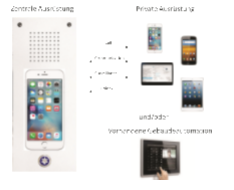
\includegraphics[height=8cm]{image/Titleimage.png}
	
	    \normalsize
	    \vspace{1cm}
	    \large \textbf{Bachelorarbeit}\\
	    \vspace{1cm}
	
	 \normalsize
	 	{
			\begin{tabular}{lll}
				\textbf{Studiengang:} & & Systemtechnik\\
				\textbf{Profil:} & & Informations- und Kommunikationssysteme\\
				\textbf{Referent:} & & Prof. Dr. Hauser-Ehninger Ulrich, MSc in Electronic Engineering\\
				\textbf{Korreferent:} & & Toggenburger Lukas, Master of Science FHO in Engineering\\
			\end{tabular}
	    }
    \end{center}
\end{titlepage}

\cleardoublepage
% \part im Inhaltsverzeichnis nicht nummerieren
\makeatletter
\let\partbackup\l@part
\renewcommand*\l@part[2]{\partbackup{#1}{}}

% leere Seite einfügen nach dem Titel
\thispagestyle{empty}
\quad 
\newpage

\pagenumbering{Roman}
\pagestyle{plain}
\section*{Zusammenfassung}
\label{sec:zusammenfassung}
%\addcontentsline{toc}{section}{Zusammenfassung}


In dieser Bachelorarbeit geht es darum ein Werkzeug/Tool zu entwickeln, das Propeller-Motor-Systeme von Leicht- bis Ultraleichtflugzeugen, sowie von Motorschirmen analysieren bzw. optimieren kann. Das Werkzeug soll weiterführende Erkenntnisse über Propeller und deren Einsatzbereich zur Verfügung stellen. Dazu werden Geometrieinformationen des Propellers von einem CAD-Programm ins Werkzeug geladen und ausgewertet. Gegebenenfalls können auch Geometrieänderungen, im Wesentlichen Änderungen an der Verdrillung des Propellers, vorgenommen werden. Anschliessend kann das Rotorsystem durch Berechnung und graphische Darstellung der Ergebnisse für verschiedene Flugsituationen ausgelegt bzw. optimiert werden. 
\\
Im Zentrum der Arbeit stand das Implementieren der Propellertheorie, welche einerseits die Blade Element Theorie und andererseits die Momentum Theorie beinhaltet, sowie das Einbinden eines Hilfsmittels, welches notwendige Koeffizienten zur Propellerberechnung liefert. Somit ermöglicht das Werkzeug dem Benutzer Schub, Drehmoment und weitere Grössen eines Propellers in verschiedenen Flugsituationen zu berechnen und damit Analysen durchzuführen. Konkret wurde das Werkzeug mit \MATLAB\cite{matlab} und Python\cite{python} umgesetzt.
\\
Ebenfalls wurde eine Verifikation mit Messdaten der Firma Helix Carbon GmbH durchgeführt, welche Hinweise auf die Richtigkeit der Berechnung gab. Auch wurden einige Beispiele zur Optimierung und zur Auslegung durchgeführt, um mögliche Anwendungsfälle aufzuzeigen.

\section*{Abstract}
\label{sec:abstract}
%\addcontentsline{toc}{section}{Abstract}

This bachelor’s thesis is about to develop a tool, which can analyze, respectively optimize propeller-engine-systems from light to ultralight aircrafts and from paramotors. The goal was to create a tool, which provides further findings about propellers and their application area. Therefore, the given propeller geometry information from a CAD program is loaded and analyzed in the tool. There can also be made optionally geometry changes, substantially changes made to the twist of the propeller. Subsequently, the rotor system can be designed and optimized by calculation and graphical representation of the results for different flight situations.\\

The main topic of the work was the implementation of the propeller’s theory, which is on the one hand the blade element theory and on the other hand the momentum theory as well as the inclusion of an auxiliary tool, which provides necessary coefficients for the propeller calculation. This allows the user to calculate and to perform analysis of thrust, torque and other values of a propeller in different flight situations. Specifically, the tool was implemented with \MATLAB\cite{matlab} and Python\cite{python}.\\

There was also carried out verification with measurements of Helix Carbon GmbH, which gave evidence on the accuracy of the calculation. Some examples for optimization and analysis were explained in order to highlight possible applications.




\newpage

% leere Seite einfügen
\thispagestyle{empty}
\quad 
\newpage
%%Inhaltsverzeichnis
\tableofcontents
\newpage

%%Seitennummerierung neu beginnen, Zahlen [arabic], röm.Zahlen [roman,Roman], Buchstaben [alph,Alph]
\pagenumbering{arabic}
\newpage
\pagestyle{fancy}






\section{Einleitung}
\label{sec:einleitung}

List Example:
\begin{itemize}
\item Maximaler Schub beim Starten z.B. wegen kurzer Startbahn
\item Maximale Fluggeschwindigkeit erreichen z.B. bei Rettungsflügen oder Ähnlichem
\item Maximale Effizienz z.B. um möglichst lange Flugzeiten zu ermöglichen
\end{itemize}



Bild Beispiel:
\vspace{0.05cm}

\begin{figure}[htb!]
	\begin{center}
		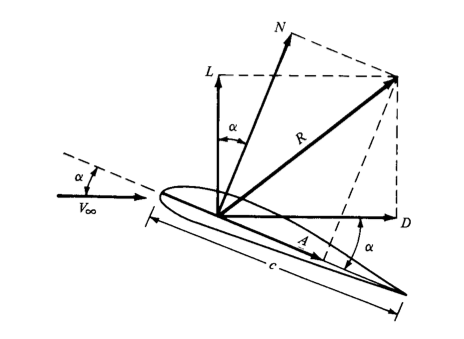
\includegraphics[width=0.48\textwidth]{airfoilKraefte}
		\caption[Wirksame aerodynamische Kräfte an einem Profil]{Wirksame aerodynamische Kräfte an einem Profil \cite{aeroKraefte}. Die Auftriebskraft $L$ wirkt beim Propeller als Schub und die Widerstandskraft $D$ als Drehmoment.}
		\label{fig:airfoilKraefte}
	\end{center}
\end{figure}

\vspace{0.05cm}

Unterkapittel:

\subsection{Subsection test}
\label{subsec:speichernderresultatematlab}

Wenn die Propellerberechnung beendet ist, werden alle Resultate in eine Baumstruktur gespeichert. Somit sind die Resultate schnell wieder aufrufbar und auch sauber in einer einzigen Datei geordnet und gespeichert.\\

\subsubsection{Subsubsection test}
\label{subsubsec:speichernderresultatematla2}

Wenn die Propellerberechnung beendet ist, werden alle Resultate in eine Baumstruktur gespeichert. Somit sind die Resultate schnell wieder aufrufbar und auch sauber in einer einzigen Datei geordnet und gespeichert.\\

\subsubsection{Subsubsubsection test}
\label{subsubsec:speichernderresultatematlab3}

Wenn die Propellerberechnung beendet ist, werden alle Resultate in eine Baumstruktur gespeichert. Somit sind die Resultate schnell wieder aufrufbar und auch sauber in einer einzigen Datei geordnet und gespeichert.\\

\newpage



\section{Chapter Example}
\label{sec:chapterexample}


Um Berechnungen rund um das Thema Propeller durchführen zu können, ist es nötig, die sogenannte Blade- und Momentum-Theorie zu verstehen und diese anwenden zu können. Die Ausführungen in dieser Arbeit orientieren sich stark an der Master-Thesis von Mario Heene\cite{heene}. Ebenfalls werden die wichtigsten Begriffe der Aerodynamik und Propellertheorie erläutert. 
\subsection{Underchapter Example}
\label{subsec:underchapterexample}

Die Gestalt von Propellern kann durch viele 2D-Profile beschrieben werden. 2D-Profile gleichen dem Querschnitt eines Flügels. Durch den geringeren Druck auf der Oberseite des Profils resultieren Kräfte, die das Profil hoch drücken (siehe Kapitel \ref{subsec:momentumtheorie}, Einschub Bernoulli) oder im Falle des Propellers, Schub erzeugen. Für jedes Profil können die Kräfte dargestellt werden.

\vspace{0.05cm}

\begin{figure}[htb!]
\begin{center}
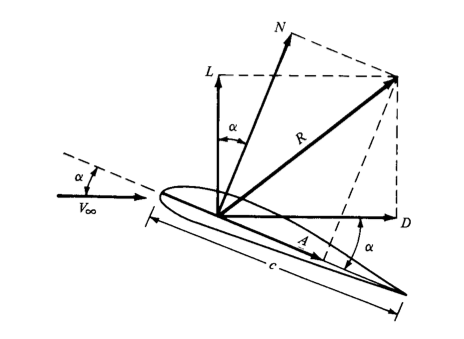
\includegraphics[width=0.48\textwidth]{airfoilKraefte}
\caption[Wirksame aerodynamische Kräfte an einem Profil]{Wirksame aerodynamische Kräfte an einem Profil \cite{aeroKraefte}. Die Auftriebskraft $L$ wirkt beim Propeller als Schub und die Widerstandskraft $D$ als Drehmoment.}
\label{fig:airfoilKraefte}
\end{center}
\end{figure}

\vspace{0.05cm}

In Abbildung \ref{fig:airfoilKraefte} sind die verschiedenen Kräfte dargestellt. $V_\infty$ stellt die Geschwindigkeit der Luft weit weg vom Körper dar. Die Kraft $R$ setzt sich zusammen aus der Auftriebskraft $L$ ('lift') und der Widerstandskraft $D$ ('drag'), wobei $L$ senkrecht zu $V_\infty$ steht und $D$ in die gleiche Richtung zeigt wie $V_\infty$.
Die Sehnenlänge $c$ ('chord') definiert die Länge des Profils von der Profilspitze bis zur Hinterkante. Dabei steht die Kraft $N$ senkrecht zu $c$ und $A$ in Richtung $c$. Der Winkel $\alpha$ ist der Winkel zwischen $V_\infty$ und $c$.
Über trigonometrische Funktionen können die Kräfte $N$ und $A$ folgendermassen beschrieben werden:





%%Verzeichnis aller Bilder


%%Literaturverzeichnis
\newpage
\bibliography{lit}
\bibliographystyle{plain}
\addcontentsline{toc}{section}{Literaturverzeichnis}
\newpage

%% Abbildungsverzeichnis, Tabellenverzeichnis, Abkürzungsverzeichnis
\listoffigures
\addcontentsline{toc}{section}{Abbildungsverzeichnis}
\newpage
\listoftables
\addcontentsline{toc}{section}{Tabellenverzeichnis}
\newpage

\thispagestyle{plain}
\section*{Abkürzungsverzeichnis}
\addcontentsline{toc}{section}{Abkürzungsverzeichnis}

\begin{acronym}[Bash]
 \acro{GUI}{Graphical User Interface}
 \acro{IP}{Internet Protocol address}
\end{acronym}
\newpage
\thispagestyle{plain}

%\begin{center}
%\begin{minipage}[t]{1\textwidth}
\section*{Eidesstattliche Erklärung}
\addcontentsline{toc}{section}{Eidesstattliche Erklärung}
Die Verfasser dieser Bachelorarbeit, Fabiano Sala und Gabriel Salkim, bestätigen, dass sie die Arbeit selbstständig und nur unter Benützung der angeführten Quellen und Hilfsmittel angefertigt haben. Sämtliche Entlehnungen sind durch Quellenangaben festgehalten.
	
	
\vspace{2cm}

\hspace{2cm} Ort, Datum \hfill Gabriel Salkim \hspace{2cm}

\vspace{4cm}

\hspace{2cm} Ort, Datum \hfill Fabiano Sala \hspace{2cm}
%\end{minipage}
%\end{center}






% leere Seite einfügen
\thispagestyle{empty}
\quad 
\newpage

\end{document}
% ======================================= Dokumentende =======================================